\documentclass[10pt,a4paper]{report}
\usepackage[utf8]{inputenc}
\usepackage[T1]{fontenc}
\usepackage{amsmath}
\usepackage{amsfonts}
\usepackage{amssymb}
\usepackage{graphicx}
\usepackage{subfloat}
\usepackage{subfig}
%\usepackage{xcolor}
\usepackage[dvipsnames]{xcolor}
\usepackage{geometry}
\geometry{a4paper, margin=0.8in}
\begin{document}
	\chapter{Version}
	This document is a common guide but it applies mainly to version $12$ or $v12$.
	
	\chapter{Components}
	\begin{figure}
		\subfloat[]{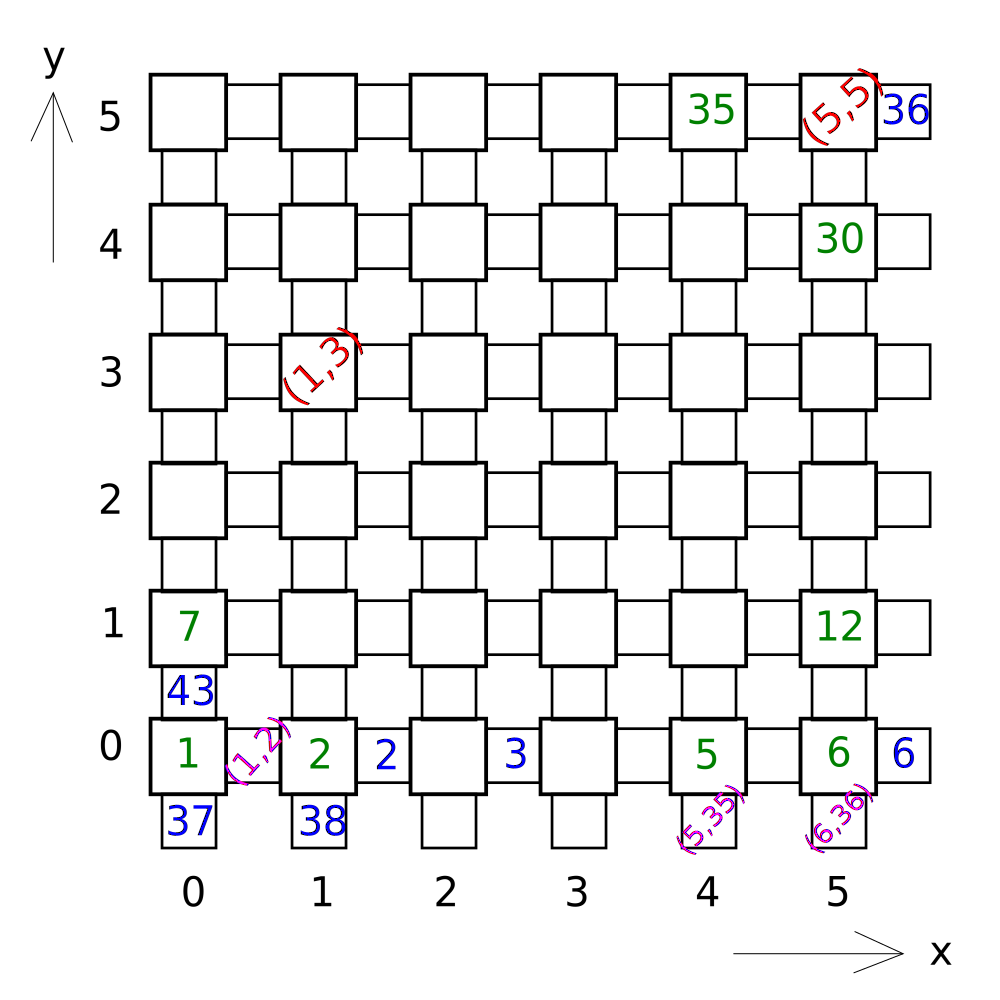
\includegraphics[width=0.8\linewidth]{fig/lattice-2.png}}
		\caption{\textcolor{red}{Red} color is for site index, \textcolor{ForestGreen}{Green} color is for site id(or label), \textcolor{magenta}{Magenta} color is for bond index, \textcolor{blue}{Blue} color is for bond id (or label).}
	\end{figure}
	\section{Site}
	\begin{enumerate}
		\item $id$ or $label$
		\item $group\_id$
		\item Index
		\item Relative Index with respect to 
	\end{enumerate}
	\section{Bond}
\begin{enumerate}
	\item $id$ or $label$
	\item $group\_id$ which can coincide with site group id
	
	\item Index. $(a,b)$ where $a$ is the $id$ of one site and $b$ is the id of another site.
\end{enumerate}
\newpage
	\section{Lattice}
	We will study $2D$ system specifically with a $2d$ vector in C++.
	\begin{enumerate}
		\item Site.
		\item Bond
	\end{enumerate}
 All the information of sites and bonds must be accessed through lattice.
	
	A $1d$ vector looks like
	\begin{equation*}
	V_i = 
	\left[
	\begin{tabular}{c}
		0 \\ 1 \\ 2
	\end{tabular}
	\right]
	\end{equation*}
	
		A $2d$ vector looks like
	\begin{equation*}
	V_{i,j} = 
	\left[
	\begin{tabular}{cccc}
	0,0 & 0,1 & 0,2 \\
	1,0 & 1,1 & 1,2 \\
	2,0 & 2,1 & 2,2
	\end{tabular}
	\right]
	\end{equation*}
	
	But we want grid like structure 
	\begin{equation*}
	V^\prime_{i,j} = 
	\left[
	\begin{tabular}{cccc}
	0,2 & 1,2 & 2,2 \\
	0,1 & 1,1 & 2,1 \\
	0,0 & 1,0 & 2,0
	\end{tabular}
	\right]
	\end{equation*}
	where each column of $V^\prime$ is row of $V$ but backwards. So when viewing the lattice we just need to generate row index backward and  switch row and column index. Note that horizontal bonds become vertical and vice versa in this process.

	\section{Cluster}
	A cluster contains site and bond ids as a list. So that when asked which site or bond it contains, cluster class can return the list.
	\begin{enumerate}
		\item site id list
		\item bond id list
		\item group id or $gid$. This is very important. All site and bonds must have this same $gid$ through which we can determine which cluster a particular site or bond belongs to.
	\end{enumerate}

	\section{Relative Index}
	To detect wrapping relative index is very useful. This only applies to sites. Relative index is the relative position of sites with respect to the root site (first site of a cluster).
	
	
	Expression is $g_{id} (x_r,y_r)$ where subscript $r$ indicates relative index. Relative index have default value $(0,0)$.
	
	\begin{figure}
		\centering
		\subfloat[\label{relative-index-2}]{\includegraphics[width=0.3\linewidth]{fig/relative-index/relative-index-2.png}}
		\subfloat[\label{relative-index-3}]{\includegraphics[width=0.3\linewidth]{fig/relative-index/relative-index-3.png}}
		\subfloat[\label{relative-index-4}]{\includegraphics[width=0.3\linewidth]{fig/relative-index/relative-index-4.png}}
		\caption{Relative index of any site is by default is $(0,0)$ even if they have different group id (\ref{relative-index-2}). Say we relabel $2$ with respect to $1$ then we get (\ref{relative-index-3}). And if the cluster grows a bit it might look like (\ref{relative-index-4}).}
	\end{figure}

\subsection{cluster relabeling by relative index}
For relative index transformation we just need the relative index of two neighbor of different cluster. Say cluster $i$ have site with relative index $(x_{ir},y_{ir})$  and coordinate index $(x_{ic},y_{ic})$ and cluster $j$ have site $(x_{jr},y_{jr})$ and coordinate index $(x_{jc},y_{jc})$.
With appropriate transformation the relative index of cluster $j$ will be changed by
\begin{equation}
\begin{split}
	x_j &\rightarrow x_j + \Delta x_r + \Delta x_c \\
	y_j &\rightarrow y_j + \Delta y_r + \Delta y_c \\
\end{split}
\end{equation}
Simplifying
\begin{equation}
\begin{split}
	x_j &\rightarrow x_j + \Delta x \\
	y_j &\rightarrow y_j + \Delta y \\
\end{split}
\end{equation}
With
\begin{equation}
\begin{split}
\Delta x &= \Delta x_r + \Delta x_c  \\
\Delta y &= \Delta y_r + \Delta y_c  \\
\end{split}
\end{equation}
Where
\begin{align}
\begin{split}
\Delta x_r &= x_{ir}-{x_jr}  \\
\Delta y_r &= y_{ir}-{y_jr}  \\
\end{split}
\\
\begin{split}
\Delta x_c &= -x_{ic}+{x_jc} \\
\Delta y_c &= -y_{ic}+{y_jc}  \\
\end{split}
\end{align}

This is demonstrated in figure (\ref{fig:relative-index-2}, \ref{fig:relative-index-3}) where $i$ is the green cluster and $j$ is the blue cluster. 

	\begin{figure}
	\centering
	\subfloat[\label{relative-index-5}]{\includegraphics[width=0.4\linewidth]{fig/relative-index/relative-index-5.png}}
	\subfloat[\label{relative-index-6}]{\includegraphics[width=0.4\linewidth]{fig/relative-index/relative-index-6.png}}
	\caption{Suppose we have two large cluster $1$ and $2$ which is indicated by green and blue color in the figure (\ref{relative-index-5}). A third site (red) is occupied which has group id $5$ and default relative index (\ref{relative-index-6}) and we decide to connect it with blue cluster then it's relative index will change from $(0,0)$ to $(0,2)$ according to it's neighbor $2(0,1)$.
	}
	\label{fig:relative-index-2}
\end{figure}
\begin{figure}
	\centering
	\subfloat[\label{relative-index-7}]{\includegraphics[width=0.4\linewidth]{fig/relative-index/relative-index-7.png}}
	\subfloat[\label{relative-index-8}]{\includegraphics[width=0.4\linewidth]{fig/relative-index/relative-index-8.png}}
	\caption{ Thus we have blue cluster of size $4$ and group id $2$ (\ref{relative-index-7}).  Then we need to merge blue and green cluster together. Green neighbor of $1(1,0)$ is $2(0,2)$. The transformation of is $2(0,2)$ goes to $1(2,0)$, i.e., we add $(\Delta x, \Delta y)=(2,-2)$ to all the element of blue cluster and we are done (\ref{relative-index-8}). Here $\Delta x_r=1$ and $\Delta y_r=-2$ for relative index difference and $\Delta x_c=1$ and $\Delta y_c=0$ for coordinate index difference.}
	\label{fig:relative-index-3}
\end{figure}

\subsection{Detect Wrapping using relative index}
Wrapping detection is done using relative index. In fact this is the only reason behind using relative index.

 At some state lattice can reach a state like (\ref{relative-index-9}) where just one site at index $(2,5)$ can trigger wrapping. We mark it by red color (\ref{relative-index-10}) which is relabeled by site at index $(3,5)$ with relative index $(1,-4)$. The red site becomes green by relative index transformation and acquires new relative index $(1,-5)$. Note that Index of any site is unchanged only relative index changes. Now we compare neighbor sites of new site indexed $(2,5)$. One is showed in figure (\ref{relative-index-11}), we can easily see that the absolute value of difference between $y$ value of the relative index is greater than $1$ which indicates that the cluster wrapped around the lattice once vertically. If absolute value of difference between $x$ values were greater than $1$ then we would say it is a horizontal wrapping.
\begin{figure}
	\centering
	\subfloat[\label{relative-index-9}]{\includegraphics[width=0.34\linewidth]{fig/relative-index/relative-index-9.png}}
	\subfloat[\label{relative-index-10}]{\includegraphics[width=0.34\linewidth]{fig/relative-index/relative-index-10.png}}
	\subfloat[\label{relative-index-11}]{\includegraphics[width=0.34\linewidth]{fig/relative-index/relative-index-11.png}}
	\caption{}
	\label{fig:relative-index-4}
\end{figure}

\chapter{Calculating Entropy Efficiently}
	There are three different ways of calculating Shannon entropy. Theoretically all are equivalent but due to computer precision these different methods are slightly different which is visible when calculating specific heat, i.e., derivative of entropy.
	\section{method 1: Slow Entropy measuring}
	In this method one just perform the sum over all cluster to get the entropy by using the definition for Shannon entropy.
	\begin{equation}
		H = - \sum_{i}^{n} \mu_i \log \mu_i
		\label{eqn.shannon-entropy}
	\end{equation}
	where $n$ is the number of cluster and $\mu_i = \frac{\text{size of i-th cluster}}{\text{sum of size of all cluster}}$ is the cluster picking probability.
	
	Although this method is the slowest but it is the most accurate if suitable data type is used, e.g. $long\ double$ in $C++$.
	
	\section{method 2: Fastest entropy measuring}
	At each step of percolation process we join smaller clusters to one big cluster and thus entropy changes. Say cluster $A_i : i={10,11,12,13}$'s are merged together to form cluster $B$ then we can subtract entropy for $A_i : i={10,11,12,13}$ and add entropy for $B_j : j = {10}$ to the total entropy. This method is the fastest and theoretically is the same but due to computer precision it may give a slightly different result for large system. This is visible if we calculate specific heat.
	
	\section{method 3}
	We create a list of size $n$, where $n$ is the maximum number of cluster the system can have. We store $i$-th value of the sum in equation (\ref{eqn.shannon-entropy}) to the $i$-th element of this list and call it $entropy_list$. 
	Now if we perform a sum over all the elements of this array then we get the total entropy.
	
	If we are to merge $A_i : i={10,11,12,13}$ clusters to cluster $B_j : j = {10}$ then we set $i={10,11,12,13}$-th element of $entropy_list$ to zero and merge the clusters. Then we calculate the entropy for $B_j$ cluster and store it in the $j$-th element.
	
	Note that if $i={10,11,12,13}$ then $j$ will be one of these $i$ indices, meaning out of the four element that we have set to zero, one will regain a non zero value.
	
	\section{Time comparison}
	\begin{table}
		\centering
		\begin{tabular}{c|c|c|c}
			length & method &  time (sec) & accuracy \\
			\hline
			$200$ & $1$ & $62$ & best\\
			$200$ & $2$ & $0.122$ &	--\\
			$200$ & $3$ & $3.84$ & to be measured
		\end{tabular}
	\caption{comparison of different entropy calculation methods}
	\end{table}

\end{document}